\chapter{Álcoois e fenóis}
Iniciando a análise de substâncias orgânicas além de hidrocarbonetos, trataremos aqui sobre álcoois e fenóis, duas funções que apresentam, ao mesmo tempo, semelhanças e diferenças: semelhança pela presença de um grupo OH (hidroxila) e diferença pela presença de um carbono saturado ligado ao grupo OH contra a presença de um carbono aromático ligado ao grupo OH.

Podemos representar, de modo genérico, um álcool pela fórmula geral R-OH, onde R é um radical alquila (metil, etil, isopropil, entre outros) enquanto um fenol é representado pela fórmula geral ArOH, onde Ar é um radical arila (aromático), como fenil, naftil, entre outros.

Álcoois podem ser considerados uma das mais versáteis funções entre aquelas presentes em moléculas orgânicas, pois podem participar de um grande número de reações e formar várias outras funções. Em algumas reações esquematizadas abaixo, a notação \textbf{[O]} indica um reagente oxidamente genérico.

\begin{enumerate}
    \item \textbf{aldeídos}, por meio da oxidação parcial de álcoois primários;
    \begin{figure}[h]
        \centering
        \caption{Oxidação de álcool a aldeído.}
        \vspace{0.5cm}
        \includegraphics[width=0.75\linewidth]{imagens/alcool-aldeido.png}
    \label{fig:alcoolaldeido}
    \end{figure}

    \item \textbf{cetonas}, por meio da oxidação de álcoois secundários;
    \begin{figure}[h]
        \centering
        \caption{Oxidação de álcool a cetona.}
        \vspace{0.5cm}
        \includegraphics[width=0.75\linewidth]{imagens/alcoolcetona.png}
    \label{fig:alcoolcetona}
    \end{figure}

    \item \textbf{haletos de alquila}, por meio da substituição nucleofílica;
    \begin{figure}[h]
        \centering
        \caption{Substituição nucleofílica de álcoois.}
        \vspace{0.5cm}
        \includegraphics[width=1\linewidth]{imagens/alcoolhaleto.png}
    \label{fig:alcoolhaleto}
    \end{figure}

    \item \textbf{alcenos}, por meio da eliminação intramolecular;
    \begin{figure}[h]
        \centering
        \caption{Desidratação intramolecular de álcoois.}
        \vspace{0.5cm}
        \includegraphics[width=0.85\linewidth]{imagens/alcoolalceno.png}
    \label{fig:alcoolalceno}
    \end{figure}

    \item \textbf{éteres}, por meio da eliminação intermolecular;
    \begin{figure}[h]
        \centering
        \caption{Desidratação intermolecular de álcoois.}
        \vspace{0.5cm}
        \includegraphics[width=1\linewidth]{imagens/alcooleter.png}
    \label{fig:alcooleter}
    \end{figure}

    \item \textbf{ésteres}, por meio da reação de esterificação;
    \begin{figure}[h]
        \centering
        \caption{Reação de esterificação.}
        \vspace{0.5cm}
        \includegraphics[width=1\linewidth]{imagens/esterificacao.png}
    \label{fig:alcoolester}
    \end{figure}

    \item \textbf{ácidos carboxílicos}, por meio da oxidação completa de álcoois primários\footnote{Embora a oxidação total de um álcool primário seja o processo de descarboxilação oxidativa, usamos aqui o termo "completa" para diferenciar do processo de oxidação parcial de álcoois}. 
    \begin{figure}[h]
        \centering
        \caption{Oxidação total de álcoois primários.}
        \vspace{0.5cm}
        \includegraphics[width=0.85\linewidth]{imagens/alcoolacido.png}
    \label{fig:alcoolacido}
    \end{figure}
\end{enumerate}

\section{Aspectos estruturais}
Em termos estruturais, álcoois e fenóis são, simultaneamente, semelhantes e distintos, pois a presença do grupo OH ligado diretamente a um carbono saturado (álcoois) ou diretamente a um carbono aromático (fenóis) confere propriedades e reatividades distintas às duas funções.

Álcoois apresentam uma característica estrutural muito importante e que ajuda a explicar boa parte de suas propriedades: a possibilidade de formaçào de ligaçòes de hidrogênio com água. A figura \ref{fig:ligacaoh} a seguir ilustra a formação dessa ligação entre etanol (esquerda) e água (direita), explicitada pelo tracejado entre as duas moléculas. Nesta representação, o átomo de carbono é bola de cor cinza, o hidrogênio é a bola branca e o átomo de oxigênio é a bola vermelha.

 \begin{figure}[h]
	\centering
	\caption{Ligação de hidrogênio entre etanol e água, desenhada usando o software Avogadro \cite{avogadro}}
	\vspace{0.5cm}
	\includegraphics[width=0.85\linewidth]{imagens/ligacaoh.png}
	\label{fig:ligacaoh}
\end{figure}

Isoladamente, as moléculas de propanol e fenol, usadas aqui como exemplo, são analisadas sem a presença de água ou qualquer outro solvente, apenas para ilustrar os efeitos decorrentes da presença do grupo OH nas duas funções. Por uma questão de simplicidade, usaremos apenas a propriedade periódica conhecida como \textbf{eletronegatividade}, juntamente com a \textbf{ressonância}, discutida anteriormente, para explicar as diferenças no caráter ácido/base do propanol e do fenol.

Parte da análise feita nesta seção utiliza o conceito de \textbf{pKa}, uma medida da ionização de uma substância quando encontra-se em solução aquosa.

A definição conceitual de pKa é a constante de equilíbrio de ionização de um ácido fraco. É uma medida da força de um ácido fraco. Quanto menor o pKa, mais forte é o ácido.

Em termos mais simples, o pKa é o pH em que a concentração de ácido não ionizado é igual à concentração de ácido ionizado.

Por exemplo, o ácido acético tem um pKa de 4,76. Isso significa que, em uma solução aquosa com pH de 4,76, a concentração de ácido acético não ionizado é igual à concentração de ácido acético ionizado. Em pHs mais baixos, o ácido acético está mais protonado, ou seja, na forma de ácido. Em pHs mais altos, o ácido acético está mais desprotonado, ou seja, na forma de base.

O átomo de oxigênio do grupo OH, nas duas funções aqui analisadas, encontra-se, inicialmente, com hibridização sp{$^3$} e confere uma relativamente elevada densidade eletrônica na região do grupo OH, conforme por ser observado nas figuras \ref{fig:fenol} e \ref{fig:propanol} a seguir, que ilustram os mapas de potencial eletrostáticos para o fenol e o propanol.

\begin{figure}[h]
    \centering
    \caption{Mapa de potencial eletrostático do fenol}
    \vspace{0.5cm}
    \includegraphics[width=0.6\linewidth]{imagens/fenol.png}
\label{fig:fenol}
\end{figure}

\begin{figure}[h]
    \centering
    \caption{Mapa de potencial eletrostático do propanol}
    \vspace{0.5cm}
    \includegraphics[width=0.75\linewidth]{imagens/propanol.png}
\label{fig:propanol}
\end{figure}

Um ponto interessante a destacar é a existência de estruturas de ressonância associadas ao íon fenolato, obtido pela ionização do fenol em água. Conforma pode ser visto na figura \ref{fig:fenolato} a seguir, a carga eletrônica inicialmente presente no átomo de oxigênio pode ser deslocalizada pelo anel aromático, o que contribui para a estabilização da estrutura como um todo.

\begin{figure}[h]
    \centering
    \caption{Estabilização do fenolato por ressonância}
    \vspace{0.5cm}
    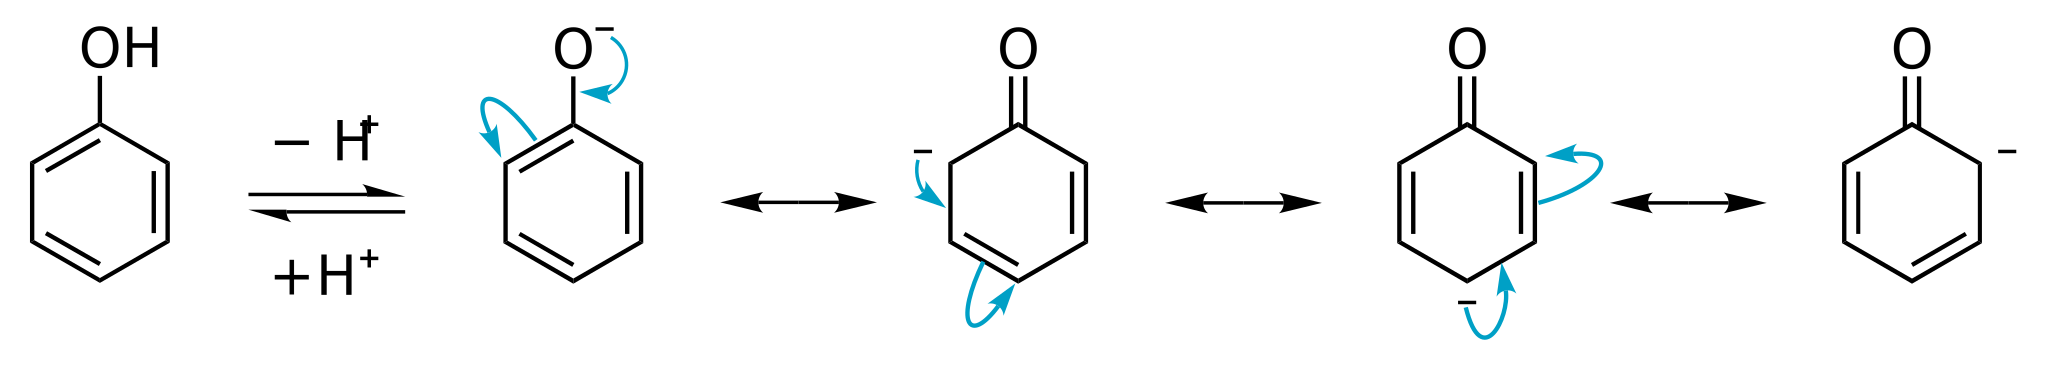
\includegraphics[width=1\linewidth]{imagens/Phenol-phenolate_equilibrium.svg.png}
\label{fig:fenolato}
\end{figure}

As setas indicadas na figura representam a movimentação de elétrons entre as diferentes formas de ressonância possíveis para o íon fenolato, e perceba que a carga negativa resultante da ionização dica deslocalizada pels estrutura.

O mesmo não ocorre no propanol e, portanto, a liberação do cátion H{$^+$} é mais difícil e o fenol apresenta caráter mais ácido que o propanol, uma vez que libera um íon hidrônio com mais facilidade, fato comprovado pelos valores de pKa do fenol (10) e do propanol (16). Uma vez que pKa é uma grandeza expressa em escala logarítmica, um elevado valor de pKa indica um ácido fraco, o que corrobora nossa análise.

Mas por que não ocorre com o propanol? Simples: a força do ácido, considerando o conceito de Brönsted-Lowry, depende da estabilidade da base conjugada, o que deixa o íon hidrônio mais livre. O pronanol não possui um sistema insaturado que permita a estabilização por ressonância.


%################################
\section{Ocorrência e aplicações}
Conforme já mencionado no início deste capítulo, álcoois e fenóis são compostos versáteis e muito úteis em diversos setores econômicos e industriais, e considerando o etanol como um dos protagonistas, por suas aplicações variando de componente de bebidas até combustíveis automotivos, passando por produtos de limpeza, tanto domésticos quanto hospitalares.

\subsection{Álcoois}
Muitos exemplos de substâncias pertencentes à função álcool possuem usos biológicos e/ou aplicações industriais e podemos fixar nossa análise em compostos monofuncionais, ou seja, possuem apenas a função álcool.

\subsubsection{Metanol}
Assim, o mais simples dos álcoois, o composto de fórmula \ce{CH3OH} recebe o nome de metanol, pois possui apenas um carbono e o hidreto pai é o metano. Pela nomenclatura substitutiva, um átomo de Hidrogênio foi substituído pelo grupo OH e álcoois possuem o sufixo ol. Justificado o nome \textbf{metanol}, certo?

\begin{figure}[h]
    \centering
    \caption{Fórmula estrutural para o metanol}
    \vspace{0.5cm}
    \includegraphics[width=0.35\linewidth]{imagens/methanol-2d-0349e4-1024.png}
\label{fig:mpemetanol}
\end{figure}

A figura \ref{fig:mpemetanol} a seguir ilustra o mapa de potencial eletrostático para o metanol e tal mapa indica a distribuição de cargas elétricas na substância, utilizando uma paleta de cores que vai do azul ao vermelho, onde este último indica maior quantidade de carga em uma dada região, comparada com a cor azul de outra região.

\begin{figure}[h]
    \centering
    \caption{Mapa de potencial eletrostático para o metanol}
    \vspace{0.5cm}
    \includegraphics[width=0.45\linewidth]{imagens/mpemetanol.png}
\label{fig:mpemetanol}
\end{figure}

Um estudo recente realizado no Brasil \cite{D2CC01757A} mostra a foto-oxidação de metano para produzir metanol em condições ambientes, catalisada por metais de transição. Comparado com métodos clássicos, as condições reacionais e a possibilidade de uso de luz solar no processo tornam esse estudo muito promissor na produção em escala industrial de metanol.

A toxicidade do metanol, indicada pelo Diagrama de Hommel, indicado na figura \ref{fig:hommel} a seguir, pode ser analisada considerando as quatro partes da imagem contendo números inteiros em uma escala entre 0 e 4, onde 0 indica ausência de problemas e 4 indica perigo crítico.

A figura geométrica do losango é usada pela NFPA (National Fire Protection Association) \footnote{Veja mais em https://www.nfpa.org/codes-and-standards/7/0/4/704}, nos Estados Unidos da América, para indicar riscos associados a cada substância cadastrada na instituição.

A parte em cor vermelha (porção superior do losango) indica a \textbf{inflamabilidade} da substância, ou seja, sua capacidade de entrar em combustão. Portanto, o metanol é bastante inflamável e com um seríssimo agravante: sua combustão gera chamas de cor azul muito claras e visíveis apenas à noite, exigindo mais cuidados em sua manipulação. Diversos acidentes envolvendo metanol já foram citados e aqueles envolvendo automóveis de corrida da chamada Fórmula Indy, categoria automobilística muito famosa nos Estados Unidos da América, são chocantes \footnote{Veja mais em https://www.essentiallysports.com/nascar-news-invisible-fire-at-the-nineteen-eighty-one-indy-five-hundred-sets-the-nascar-community-ablaze-after-fans-make-talladega-superspeedway-nights-connection/}.

A parte em cor azul (porção central e esquerda do losango) indica o \textbf{risco à saúde} e, portanto, o contato ou ingestão deve ser evitado. Para referência, a dose letal por via oral em ratos é de pouco mais de 5,6 g/kg de peso corporal.

A parte em cor amarela (porção central direita do losango) indica \textbf{instabilidade ou reatividade} e mostra a estabilidade do metanol.

A parte em cor branca (porção inferior do losango) indica \textbf{risco específico} (oxidante forte ou radioativo, por exemplo) e não há registros de tal categoria para o metanol.


\begin{figure}[h]
    \centering
    \caption{Diagrama de Hommel para o metanol}
    \vspace{0.5cm}
    \includegraphics[width=0.25\linewidth]{imagens/hommel.png}
\label{fig:hommel}
\end{figure}

\subsubsection{Etanol}
Este álcool possui tamanha importância no Brasil, seja como combustível, como componente de produtos de limpeza ou em bebidas alcoólicas, que seu nome se confunde com a função orgânica à qual pertence. Por muito tempo os brasileiros compravam "álcool" em postos de combustíveis e apenas recentemente a substância passa a ser comercializada com seu nome oficial.

Trata-se de um líquido transparente, incolor, com densidade em torno de 0,8 g/cm$^3$ e miscível com água em qualquer proporção, explicado por meio da formação de ligações de hidrogênio entre água e etanol de modo tão intenso, que a mistura líquida é classificada como azeótropo, ou seja, os componentes da mistura entram em ebulição juntos, o que inviabiliza a destilação comum como meio de separação dos componentes desta mistura. Porém, é possível separar os componentes da mistura por outros métodos \cite{trica}.

\begin{figure}[h]
	\centering
	\caption{Diferentes representações para o etanol}
	\vspace{0.5cm}
	\includegraphics[width=0.75\linewidth]{imagens/etanol2.jpeg}
	\label{fig:etanol2}
\end{figure}

A figura \ref{fig:etanol2} ilustra ao menos duas representações distintas para o etanol: a fórmula estrutural completa (esquerda) e a representação do tipo "ball \& stick" (tubo e bola) (direita), onde as bolinhas de cores e/ou tamanhos diferentes representam os átomos e os tubinhos representam as ligações químicas entre eles. Existem diferentes representações para moléculas orgânicas em função do contexto de uso, onde uma dada representação pode ser mais esclarecedora que outra.

No Brasil, o etanol é produzido, essencialmente, por fermentação de sacarose por meio de leveduras, em inúmeras usinas de produção espalhadas pelo país, fato que movimenta um enorme número de trabalhadores nos diversos segmentos de produção e distribuição, alimentando uma cadeia produtiva bastante ampla.

Como é produzido a partir da sacarose obtida pela cana-de-açúcar, parte do dióxido de carbono, CO$_2$, produzido pela queima do etanol em motores a combustão, podemos dizer que o etanol é um combustível de ciclo neutro, conforme pode ser visto na figura \ref{fig:neutro} a seguir

 \begin{figure}[h]
 	\centering
 	\caption{Etanol como combustível de ciclo neutro}
 	\vspace{0.5cm}
 	\includegraphics[width=1\linewidth]{imagens/ciclo-neutro.png}
 	\label{fig:neutro}
 \end{figure}

\subsection{Fenóis}
Fenóis são encontrados em muitas fontes vegetais, sendo responsáveis (em parte) pela coloração de flores, frutas e alguns tecidos vegetais, muitas vezes na forma de flavonóides, um tipo de polifenóis bastante comum em plantas, como pode ser visto na figura \ref{fig:taxi} a seguir.

\begin{figure}[h]
    \centering
    \caption{Exemplo de flavonóide: taxifolina.}
    \vspace{0.5cm}
    \includegraphics[width=0.6\linewidth]{imagens/taxifolina.png}
\label{fig:taxi}
\end{figure}

As substâncias pertencentes à função fenol são muito utilizadas biologicamente \cite{doi:10.1021/acs.jmedchem.2c00223}, pois podem apresentar ação:

\begin{itemize}
    \item antioxidante: qualquer substância capaz de impedir ou retardar reações de degradação oxidativa (Figura \ref{fig:toco}), seja por meio da inibição de radicais livres (muito comuns em processos oxidativos) ou então pela formação de complexos metálicos (cátions metálicos formando ligações coordenadas ou dativas com outros íons ou moléculas). 

    \begin{figure}[H]
        \centering
        \caption{Exemplo de fenol com ação anti-oxidante}
        \vspace{0.5cm}
        \includegraphics[width=1\linewidth]{imagens/tocoferol.png}
    \label{fig:toco}
    \end{figure}
    \item antitumoral: O termo "ação antitumoral" refere-se à capacidade de uma substância ou tratamento de inibir ou neutralizar o crescimento e o desenvolvimento de tumores, que são massas anormais de tecido resultantes da divisão celular descontrolada. As ações antitumorais podem ser observadas em vários níveis, visando diferentes aspectos dos processos complexos envolvidos na tumorigênese \footnote{A tumorigênese é o ganho de propriedades malignas em células normais, incluindo principalmente desdiferenciação, proliferação rápida, metástase, evasão da apoptose e imunovigilância, metabolismo desregulado e epigenética, etc., que foram generalizadas como as características do câncer}.
    \begin{figure}[H]
        \centering
        \caption{Exemplo de fenol com ação antitumoral}
        \vspace{0.5cm}
        \includegraphics[width=0.5\linewidth]{imagens/dr.png}
    \label{fig:doxo}
    \end{figure}
    \item antimicrobiana: A ação antimicrobiana refere-se à capacidade de uma substância ou agente de inibir ou matar micro-organismos, como bactérias, vírus, fungos ou protozoários. Esta ação é crucial em vários contextos, incluindo medicina, saúde e preservação de alimentos e outros produtos. Os agentes antimicrobianos podem ser naturais ou sintéticos e são projetados para atingir tipos específicos de microrganismos.
    \begin{figure}[H]
        \centering
        \caption{Exemplo de fenol com ação antimicrobiana}
        \vspace{0.5cm}
        \includegraphics[width=0.65\linewidth]{imagens/triclosan.png}
    \label{fig:triclosan}
    \end{figure}
    \item anti-inflamatória: A ação anti-inflamatória refere-se à capacidade de uma substância ou tratamento de reduzir a inflamação no corpo. A inflamação é uma resposta natural e necessária do sistema imunológico a lesões ou infecção. No entanto, a inflamação crônica ou excessiva pode contribuir para várias condições de saúde, incluindo doenças autoimunes e distúrbios inflamatórios crônicos.

    \begin{figure}[H]
        \centering
        \caption{Exemplo de fenol com ação anti-inflamatória}
        \vspace{0.5cm}
        \includegraphics[width=0.45\linewidth]{imagens/cresotico.png}
    \label{fig:cresotico}
    \end{figure}
    \item anti-hemorrágica: A ação anti-hemorrágica refere-se à capacidade de uma substância ou tratamento de prevenir ou controlar o sangramento. Hemorragia é o termo médico para sangramento excessivo, que pode ocorrer interna ou externamente e pode ser resultado de várias condições ou lesões. Ações anti-hemorrágicas podem ser alcançadas por meio de diferentes mecanismos, e várias substâncias ou intervenções podem exibir essa propriedade \cite{SOUZA2022105299}.
    
    \begin{figure}[H]
        \centering
        \caption{Exemplo de fenol com ação anti-hemorrágica}
        \vspace{0.5cm}
        \includegraphics[width=1\linewidth]{imagens/caju.png}
    \label{fig:caju}
    \end{figure}
\end{itemize}

Porém, nem todos os fenóis apresentam ação biológica benéfica. A substância ácido piridina2,3-dicarboxílico, apresentada na figura \ref{fig:4hexil} apresenta ação neurotóxica, enquanto a outra substância ma mesma imagem apresenta ação antitumoral.

\begin{figure}[ht]
    \centering
    \caption{Exemplos de fenóis com ação biológica}
    \vspace{0.5cm}
    \includegraphics[width=1\linewidth]{imagens/res.png}
\label{fig:4hexil}
\end{figure}

O fenol mais simples conhecido, chamado inicialmente de \textbf{ácido carbólico}, foi utilizado em conjunto (e depois isoladamente) para extermínio em massa de prisioneiros em campos de concentração alemães durante a II Guerra Mundial, por meio de injeção direta no coração dos prisioneiros \cite{triste}.

%#####################
\section{Nomenclatura}
A nomenclatura de compostos monofuncionais da função álcool é bem simples e segue o padrão já visto anteriormente neste texto, considerando a posição do grupo funcional hidroxila para iniciar a numeração da cadeia carbônica. Veja os exemplos a seguir, discutidos caso a caso.

\begin{tcolorbox}[colback=white!5!white,colframe=orange!90!black,title=\textbf{Exemplo 1}]
	\begin{figure}[H]
		\centering
		%\vspace{0.5cm}
		\includegraphics[width=0.3\linewidth]{imagens/isopropanol.png}
		\label{fig:isopropanol}
	\end{figure}
	\tcblower
    A imagem representa um álcool com cadeia carbônica saturada e, portanto, o hidreto pai é chamado de \textbf{propano}. Existe um grupo funcional na posição 2 da cadeia carbônica e, utilizando a nomenclatura substitutiva, a molécula recebe o nome de \textbf{propan-2-ol}, conhecido também pelo nome de \textbf{álcool isopropílico}.
\end{tcolorbox}

\begin{tcolorbox}[colback=white!5!white,colframe=orange!90!black,title=\textbf{Exemplo 2}]
	\begin{figure}[H]
		\centering
		%\vspace{0.5cm}
		\includegraphics[width=0.20\linewidth]{imagens/ciclopentanol.png}
		\label{fig:ciclopentanol}
	\end{figure}
	\tcblower
	A imagem representa um álcool com cadeia carbônica saturada e cíclica com cinco átomos de carbono, e, portanto, o hidreto pai é chamado de \textbf{ciclopentano}. Existe um grupo funcional na posição 1 da cadeia carbônica e, utilizando a nomenclatura substitutiva, a molécula recebe o nome de \textbf{ciclopentan-1-ol}. Em situações como essa, com o único grupo funcional na posição 1, a posição do localizador pode ser omitida..
\end{tcolorbox}


\begin{tcolorbox}[colback=white!5!white,colframe=orange!90!black,title=\textbf{Exemplo 3}]
	\begin{figure}[h]
		\centering
		%\vspace{0.5cm}
		\includegraphics[width=0.20\linewidth]{imagens/cpd.png}
		\label{fig:cpd}
	\end{figure}
	\tcblower
	A imagem representa um álcool com cadeia carbônica insaturada e cíclica com cinco átomos de carbono, fato que exige a posição dos localizadores e implica, naturalmente, na numeração precisa da cadeia carbônica. Como a senioridade do grupo funcional é maior que a da insaturação, a numeração começa no átomo de carbono que sustenta o grupo funcional. Neste caso, a insaturação começa na posição 3 do hidreto pai e, portanto, o nome da substância é \textbf{ciclopent-3-en-1-ol}.
\end{tcolorbox}

\begin{tcolorbox}[colback=white!5!white,colframe=orange!90!black,title=\textbf{Exemplo 4}]
	\begin{figure}[h]
		\centering
		%\vspace{0.5cm}
		\includegraphics[width=0.3\linewidth]{imagens/metilcpd.png}
		\label{fig:metilcpd}
	\end{figure}
	\tcblower
	A imagem representa uma substância muito parecida com a do Exemplo 3, mas com um substituinte que exige a posição de um localizador. Considerando que radicais devem ocupar a menor posição possível, a numeração deve prosseguir, a partir do grupo OH, para a direita e, portanto, o nome da substância é \textbf{2-metil-ciclopent-3-en-1-ol}.
\end{tcolorbox}

\begin{tcolorbox}[colback=white!5!white,colframe=orange!90!black,title=\textbf{Exemplo 5}]
	\begin{figure}[h]
		\centering
		%\vspace{0.5cm}
		\includegraphics[width=0.5\linewidth]{imagens/2metilhex.png}
		\label{fig:2metilhex}
	\end{figure}
	\tcblower
	A imagem representa um álcool com cadeia acíclica, insaturada e com um substituinte. Uma vez que a senioridade do grupo funcional é maior que a da insaturação, a numeração começa na extremidade mais próxima da posição do grupo OH. O próximo passo é indicar a posição dos localizadores e teremos o nome completo da substância: \textbf{2-metil-hex-5-en-3-ol}.
\end{tcolorbox}

\begin{tcolorbox}[colback=white!5!white,colframe=orange!90!black,title=\textbf{Exemplo 6}]
	\begin{figure}[h]
		\centering
		%\vspace{0.5cm}
		\includegraphics[width=0.45\linewidth]{imagens/dmf.png}
		\label{fig:2metilhex}
	\end{figure}
	\tcblower
	O fenol indicado na figura acima possui dois substituintes iguais e sem a presença de localizadores, o que simplifica o nome, permitindo o uso do prefixo \textbf{di} após a numeração da cadeia carbônica. Assim, o nome oficial deste fenole é \textbf{3,5-dimetilfenol}.
\end{tcolorbox}

\begin{tcolorbox}[colback=white!5!white,colframe=orange!90!black,title=\textbf{Exemplo 7}]
	\begin{figure}[h]
		\centering
		\includegraphics[width=0.3\linewidth]{imagens/pcf.png}
		\label{fig:2metilhex}
	\end{figure}
	\tcblower
	O nome deste fenol é um dos mais simples, embora não pareça. O anel benzênico suporta, no máximo, 6 substituintes diferentes e todas as posições nas quais pode haver um substituintes estão ocupadas. Temos cinco substituintes iguais (cloro) e o nome oficial da substância é \textbf{pentaclorofenol}.
\end{tcolorbox}

\begin{tcolorbox}[colback=white!5!white,colframe=orange!90!black,title=\textbf{Exemplo 8}]
	\begin{figure}[h]
		\centering
		%\vspace{0.5cm}
		\includegraphics[width=0.25\linewidth]{imagens/etilmetil.png}
		\label{fig:2metilhex}
	\end{figure}
	\tcblower
	O fenol representado acima apresenta em seu anel aromático dois substituintes diferentes: etil e metil, em posições diferentes. Considerando a regra de manter os localizadores nas menores posições numéricas possíveis, a numeração deve iniciar-se no carbono que sustenta o grupo hidroxila (OH) e então prosseguir para a direita. Substituintes diferentes devem ser citados em ordem alfabética e, assim, o nome oficial deste fenol é \textbf{4-etil-3-metil-fenol}.
\end{tcolorbox}

\begin{tcolorbox}[colback=white!5!white,colframe=orange!90!black,title=\textbf{Exemplo 9}]
	\begin{figure}[ht]
		\centering
		%\vspace{0.5cm}
		\includegraphics[width=0.5\linewidth]{imagens/propofol.png}
		\label{fig:propofol}
	\end{figure}
	\tcblower
	Esta molécula apresenta uma intensa ação anestésica e é conhecida no meio médico com o nome de \textbf{propofol}. Seu PIN (Preferred IUPAC Name) é simples: existem dois radicais iguais nas posições 2 e 6 do anel aromático e devem ser indicados, de acordo com as mais recentes recomendações através do prefixo \textbf{bis}. Mas por que não \textbf{di(propan-2-il)}? Simples: a presença de um localizador (o número 2 dentro dos parênteses) exige o uso dos parênteses e estes exigem o prefixo \textbf{bis}. Portanto, o nome oficial desta molécula é \textbf{2,6-bis-(propan-2-il)fenol}.
\end{tcolorbox}


